
\section{Empirical Methodology} 
\label{sec: emp}

%%%overview
To evaluate our method we conducted two user studies. The first was designed to
assess whether \disalg~ summaries help users identify the superior between two alternative agents, while the second user study examined whether such
summaries are useful for conveying agent behavior differences. In both studies we
use the HIGHLIGHTS algorithm as a baseline for comparison. We note here that
there is a significant difference between the output summaries of both methods
rooted in the fact that \disalg~ was designed for presenting two policies in a contrastive manner. This is achieved by portraying both agents simultaneously on the screen.
To our knowledge no other global explanation methods exist that directly compare
 policies and visualizes their differences to lay users.
% which we can compare to\footnote{\citet{Sequeira2020} propose additional
% criteria for generating alternative HIGHLIGHTS summaries, we chose to compare
% the vanilla version of the algorithm.}. 

%%%% empirical domain
\emph{Empirical Domains.} To evaluate our algorithm we generated summaries of
agents playing the game of Frogger \cite{Frogger_game} and controlling a vehicle
in a highway environment \cite{highway-env}. 

\textbf{Frogger} The objective of the game is to guide a frog from the bottom of
the screen to an empty lily-pad at the top of the screen. The agent controls the
frog and can initiate the following four movement actions: up, down, left or
right, causing the frog to hop in that direction. To reach the goal the agent
must lead the frog across a road with moving cars while avoiding being run over,
then, the agent must pass the river by jumping on passing logs. This domain
allows us to compare different agents in a setting with ground truth information
about agents' skill, i.e. game score.

\textbf{Highway} This domain consists of a busy highway with multiple lanes and
vehicles. The
agent controls a vehicle driving through traffic with the intent of avoiding
collisions. The agent can choose to move right or left (changing lanes),
increase or decrease velocity or stay idle, i.e. make no change. There is no
defined target the agent is required to reach, instead the road goes on
continuously. This property allows us to observe the agent's general behavior and preferences
instead of focusing on its progression towards reaching the goal.Screenshots from the \disalg~ output summaries displayed in Figure \ref{fig:
domains}. 


\begin{figure}[t]
	\centering
    \frame{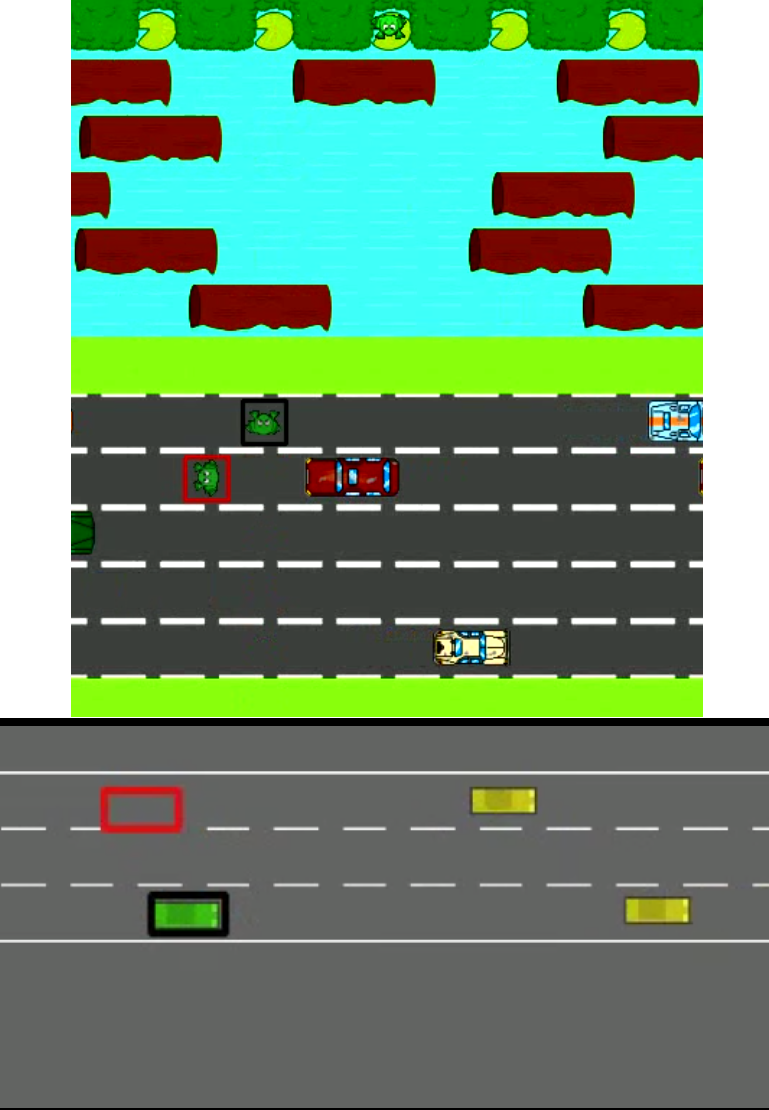
\includegraphics[width=0.7\columnwidth]{images/domains.png}}\\
	\caption{\centering{Top: Frogger; Bottom: Highway.\\ Red \& black rectangles represent different agents.}}
	\label{fig: domains}
\end{figure}

%%%% the agents
\emph{Frogger Agents.} We made use of the framework developed by
\citet{Sequeira2020} to test the \disalg~ algorithm on multiple configurable
agents of varying capabilities. Three different agents were trained using standard $Q$-learning \cite{watkins1992q}, based on the configurations provided by the framework. 
\begin{itemize}
	\item \textbf{Expert (E):} 2000 training episodes. Default rewards. Average
	game score: 110,000.
	\item \textbf{Mid-range (M):} 1000 training episodes. Default rewards.
	Average game score: 50,000.
	\item \textbf{LimitedVision (LV):} 2000 training episodes. Default rewards.
	Lower perception of incoming cars. Average game score: 55,000.
\end{itemize}
Agent performance was calculated by averaging the game score of ten
executions. Each agent's unique configuration contributes to its performance,
providing us a ground truth for the assessment tasks we present to the
experiment participants. The agents' skill hierarchy, based on their average
score, is as follows: $E>LV>M$. An important requirement for the
experiment was that all agents have a decent ability to play Frogger.
Prior to this study, we verified via an additional experiment that HIGHLIGHTS summaries are indeed useful for comparing Frogger agents that differ \emph{substantially} in their skills (see Appendix).
All HIGHLIGHTS and \disalg~ summaries were generated for fully trained agents, thus
reflecting their final policies. 


\emph{Highway Agents.}  Agents with varying behaviors were trained by altering their reward functions. All highway agents were trained for 2000 episodes using double DQN architecture
\cite{hasselt2010double} and rewarded for avoiding collisions.
\begin{itemize}
	\item \textbf{ClearLane (CL):} Rewarded for high velocity while maximizing the distance between
	itself and the nearest vehicle in front of it.
	\item \textbf{SocialDistance (SD):} Rewarded for maximizing the distance
	between itself and the closest $k$ vehicles.
	\item \textbf{FastRight(FR):} Rewarded for high velocity and driving in the
	rightmost (bottom) lane.
\end{itemize}
Henceforth,
we will refer to all domain agents by their abbreviations.

\emph{Summary Attributes}
% are listed in Table \ref{tb:parameters}. \ya{this moved to supplementary,
% mention that it's there or simply don't mention?}
All summaries were composed of five trajectories made up of sequential states, ten for Frogger and twenty for Highway. These contained the important state at the center of the
trajectory, with half the states preceding and the rest succeeding it.
Video-clips of the summaries were generated to present to the users and a
fade-in and fade-out effect was added to further call attention to the
transition between trajectories.
 For more details, sensitivity analysis and the complete surveys, see Appendix.
% \footnote{A summary of length 5
% was found useful in previous experiments with
% HIGHLIGHTS~\cite{amir18highlights}.}
% \footnote{Parameter sensitivity test appears in the Appendix.}
% \footnote{Parameter values used to generate
% summaries provided in the Appendix.}.


\paragraph{Experiment 1 - Identifying Superiority}
The objectives of the first experiment were twofold. Firstly, to support our
claims regarding the limitations of the HIGHLIGHTS algorithm for comparing
agents, and secondly, to compare the \disalg~ algorithm to HIGHLIGHTS and show
its added value. 

\emph{Hypotheses.} 
We hypothesized that summaries generated by the HIGHLIGHTS
algorithm are limited in their ability to help users distinguish between agents
and the \disalg~ algorithm is more suited for this task. More specifically,
we state the following hypotheses: \\
 \textbf{H1:} Participants shown summaries generated by HIGHLIGHTS for
 agents of decent skill will struggle to identify the better performing
 agent. \\
\textbf{H2:} Participants shown summaries generated by the \disalg~
algorithm will exhibit a higher success rate for identifying the better
performing agent, compared to ones shown HIGHLIGHTS summaries. 

%     \item \textbf{H3:} Explanation satisfaction of participants shown \disalg~
%     summaries will not be lower than that of participants shown HIGHLIGHTS
%     summaries (i.e. does not harm explanation satisfaction)\footnote{This hypothesis applies and was tested for both experiments}.
% 	\ya{maybe remove hypothesis about satisfaction?} \oa{definitely possible}



\emph{Experimental Conditions}
A between-subject experimental setup was designed with two experimental
conditions that varied in the summary generation method, \disalg~ or
HIGHLIGHTS~\cite{amir18highlights}. Participants were randomly assigned a
condition. 


\emph{Participants.} 74 participants were recruited through Amazon Mechanical
Turk (27 female, mean age $= 36.51$, STD $= 9.86$), each receiving $\$3$ for
their completion of the Task. To incentivize
participants to make an effort, they were provided a bonus of 10 cents for each
correct answer in the superiority identification task.
Participants who spent less than a threshold duration of time on experiment tasks, based on the length of the task summary video, were filtered out.

%%%% Procedure \emph{Procedure.} The experiments starts of by introducing
% participants to the game of Frogger, the concept of AI agents and to visual
% summaries as produced by HIGHLIGHTS. Each explanation was followed by a short
% quiz to ensure understanding before advancing to the task. Next, participants
% were faced with two stages of agent selection tasks, each followed by an
% explanation satisfaction questionnaire.

% \textbf{Part A: Comparing agents with a high degree of variation in skill} The
% first part of the experiment was designed to ensure that agents whose
% performance \emph{does} vary greatly are indeed distinguishable using the
% HIGHLIGHTS summaries. We further describe this task and its results in the
% supplementary material.

% \textbf{Part B: Comparing agents with a low degree of variation in skill:}  In
% this part of the experiment, 

\emph{Procedure.} Participants were first introduced to the game of Frogger and
the concept of AI agents. Each explanation was followed by a short quiz to
ensure understanding before advancing to the task. Next, participants were
randomly split into one of two conditions and were shown summary videos of pairs
of different agents generated using either \disalg~ or HIGHLIGHTS. 
% The pairs of agents shown to participants in this section were combinations of
%  $E$, $M$, $LV$ which all possess high game capabilities. (i.e. exhibit low
%  degree of variation in performance). 

Participants in both groups were first introduced to the summary method they
would be shown and were required to pass a quiz to ensure their understanding.
Participants were then asked to choose the better performing agent based on the
summary videos. They were able to pause, play and repeat the summary videos
without restrictions, allowing freedom to fully inspect the
summary before deciding which agent they believe is more skillful. Participants
were also asked to provide a textual explanation for their selection and to rate
their decision confidence on a 7-point Likert scale (0 - not at all confident to 6 - very confident). Overall, there were 3 pairs of
agent comparisons $\langle E,M\rangle \langle E,LV\rangle \langle LV,M \rangle
$. The ordering of the agent pairs was randomized to avoid learning effects, and
participants were also not told if the same agent appeared in multiple
comparisons, that is, they made each decision independently of other decisions.

% and 6 configurations when accounting for the order of the summaries shown.
% Each participant was shown one configuration of each agent pair combination,
% resulting in three overall comparisons.
Participants in the HIGHLIGHTS condition were shown a HIGHLIGHTS summary of each
agent (i.e. two separate videos, one for each agent.), while participants in the
\disalg~ group were supplied two configurations of the \disalg~ summaries. One
summary where the first agent is the Leader while the second is the Disagreer,
and the opposite summary, where the first agent is the Disagreer and the second
is the Leader. 
% That is, in both conditions participants were provided with two
% videos, each of the same number of trajectories: in the HIGHLIGHTS condition
% each video showed only one of the agents, while in the \disalg~ condition each
% video showed both agents (each with different Leader and Disagreer roles).
Upon
conclusion, participants answered a series of explanation
satisfaction questions adapted from \cite{hoffman2018metrics}. 

\emph{Evaluation Metrics and Analyses.} 
The main evaluation metric of interest was the success rate of identifying the superior Frogger agent with each summary method. We compare this metric across all the agent selection tasks given to participants. We also compare participants’ confidence in their decision.
% and show the differences between the confidence of the participants who
% succeeded in identifying the better agent using the \disalg~ algorithm
% compared to HIGHLIGHTS.
To compare the explanation satisfaction ratings given to the summaries, we
averaged the values of the different items normalizing in such a way that
higher values always mean that the summary is more helpful.
% while 1 it was not. We now report the results of the user study. We report the
% mean values and the $95\%$ confidence interval (CI) computed using the
% non-parametric Mann-Whitney $U$ test. In all plots the error bars correspond
% to the $95\%$ confidence intervals. The full experiment survey can be found in
% Appendix \ref{app: survey}
In all analyses we used the non-parametric Mann-Whitney $U$ test and computed
effect sizes using rank-biserial correlation. In all plots the error bars depict
the bootstrapped $95\%$ confidence intervals~\cite{efron1994introduction}. 
% T We use bootstrap non-parametric analysis~\cite{efron1994introduction} for
% the statistical tests. Plots show 95\% confidence intervals and we report the
% p-values for each comparison. %  but in all cases we state significant
% differences, the adjusted p-values were also smaller than 0.05. 


\begin{figure*}[t]
	\centering
	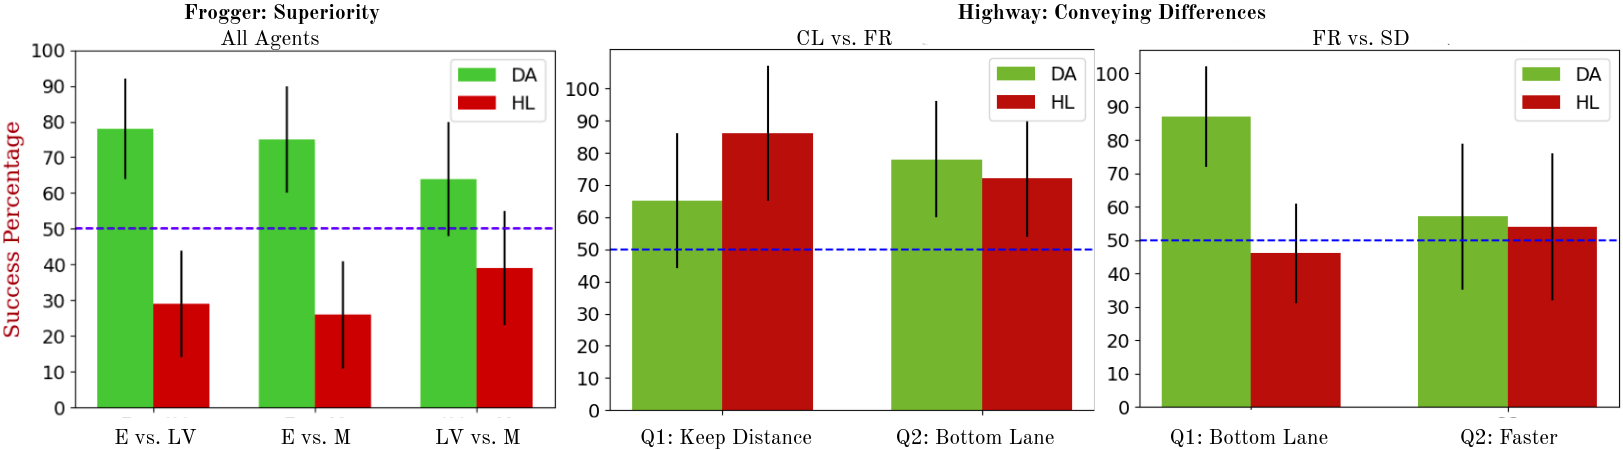
\includegraphics[width=0.85\linewidth]{images/successes_three.png}\\
	\caption{Participant Success Percentage per Summary Method. DA: DISAGREEMENTS; HL: HIGHLIGHTS.}
	\label{fig: DA HL compare}
\end{figure*}


\paragraph{Experiment 2 - Conveying Agent Differences}
This experiment's objective was to test the usefulness of \disalg~ summaries for conveying differences in general agent behavior in comparison to HIGHLIGHTS.

\emph{Hypotheses.} 
The \disalg~ algorithm is designed to portray instances of disagreement between
agents. We hypothesized that this would provide a clear and contrastive distinction between the alternative agents, thus emphasizing behavioral differences and providing a more appealing visual experience.
More specifically,we state the following hypotheses:\\ 
\textbf{H3:} Success rate of participants shown \disalg~  summaries will surpass that of participants shown HIGHLIGHTS summaries.  
\\
\textbf{H4:} participants will prefer summaries generated by the \disalg~ method.



\emph{Experimental Conditions}
A within subject setup was chosen in order to allow participants to provide a
direct comparison between the methods and state their preferences. As
participants experience both HIGHLIGHTS and \disalg~ summaries, to reduce cognitive overload, we chose to display only two agent comparisons for each
method. We chose the comparisons between the most distinctly dissimilar agents,
dropping $\langle SD,CL\rangle$ due to similarity of reward associated with
distance from neighboring vehicles. 

\emph{Participants.} 45 participants were recruited through Amazon Mechanical
Turk (13 female, mean age $= 37.51$, STD $= 10.35$), receiving similar pay and
bonus incentive as in the first experiment.
As in Exp\#1, participants were filtered out if their task completion time was below a threshold.

\emph{Procedure.} Participants followed a similar procedure as in the previous
experiment diverging solely in the domain introduction and the questions asked.
Instead of superiority between the agents, participants were queried about which
trait was more dominant in the compared agents. The ground truth was established
directly from the reward functions of the agents. Each comparison included two
such questions along with a mandatory confidence rating and textual explanation of the answers. In addition, participants were ultimately asked which method they preferred. Since this was a within-subject design, participants saw both methods, in a random order. All questions are provided in the Appendix.


\emph{Evaluation Metrics and Analyses.} 
The main evaluation metric of interest was the success rate of correctly assigning a more dominant trait to an agent. We compare this metric across the
different agent selection tasks and summary methods. Similarly to experiment 1, we compare participants’ confidence in their answers. For evaluating summary method satisfaction of participants we used the non-parametric Wilcoxon signed-rank test \cite{wilcoxon1947probability} for matched pairs.